\begin{document}

% Front matter
\frontmatter

%% r.1 blank page
%\blankpage
%
%% v.2 epigraphs
%\newpage\thispagestyle{empty}
%\openepigraph{%
%The public is more familiar with bad design than good design.
%It is, in effect, conditioned to prefer bad design, 
%because that is what it lives with. 
%The new becomes threatening, the old reassuring.
%}{Paul Rand%, {\itshape Design, Form, and Chaos}
%}
%\vfill
%\openepigraph{%
%A designer knows that he has achieved perfection 
%not when there is nothing left to add, 
%but when there is nothing left to take away.
%}{Antoine de Saint-Exup\'{e}ry}
%\vfill
%\openepigraph{%
%\ldots the designer of a new system must not only be the implementor and the first 
%large-scale user; the designer should also write the first user manual\ldots 
%If I had not participated fully in all these activities, 
%literally hundreds of improvements would never have been made, 
%because I would never have thought of them or perceived 
%why they were important.
%}{Donald E. Knuth}


% r.3 full title page
\maketitle


% v.4 copyright page
\newpage
\begin{fullwidth}
	{\large {\it Author\ \ } Vic Smith, Laith Alissa, Jon Cave, Joseph Siddall
	
	\vspace{1em}\noindent{\it Supervisor\ \ } Sara Kalvala
	
	\vspace{1em}\noindent{\it Abstract\ \ } Bla, bla, bla, abstract...
	
	\vspace{1em}\noindent{\it Keywords\ \ } Functional Programming, Haskell, Games, etc
	
	}
	
	~\vfill
	\thispagestyle{empty}
	\setlength{\parindent}{0pt}
	\setlength{\parskip}{\baselineskip}
	Copyright \copyright\ \the\year\ \thanklessauthor
	
	\par\smallcaps{Published by \newlinetospace{\thanklesspublisher}}
	
	%\par\smallcaps{Typesetting: tufte-latex.googlecode.com}
	
	\par\textit{First printing, \monthyear}

	\newpage

% r.5 contents
\tableofcontents

\end{fullwidth}
%\listoffigures

%\listoftables

%\lstlistoflistings

 %r.7 dedication
%\cleardoublepage
%~\vfill
%\begin{doublespace}
%\noindent\fontsize{18}{22}\selectfont\itshape
%\nohyphenation
%Dedicated to...
%\end{doublespace}
%\vfill
%\vfill


%%
% Start the main matter (normal chapters)
\mainmatter

% r.9 introduction
%\chapter[Foreword]{Foreword}
\label{ch:forward}

\chapterepigraph{``Perhaps it hasn't one," Alice ventured to remark. ``Tut, tut, child!" said the Duchess. ``Everything's got a moral, if only you can find it."}{from Lewis Carol's  \emph{Alice in Wonderland}}

\newthought{Starting a sentance} with a newthought.

\section{A Section}

Lorum ipsum dolor sit amet.
%\input{chapter/frontmatter/brief}

%\part{Project Specification\label{part:spec}}
	\chapter[Introduction]{Introduction}
\label{ch:motivation}

\chapterepigraph{If you aren't sure which way to do something, then do it both ways and see which works better.}{John Carmack}

\newthought{Functional programming} (FP) has a long history, with its roots in the $\lambda$-calculus of Alonzo Church.\citefix[-1.5em]{church1932} One of the first functional programming languages was Lisp, invented by John McCarthy in 1958, which is still used today, over 50 years later.\citepage{reilly2003}{pages 156--157} Various languages have refined and extended the functional paradigm over the years --- probably the most notable as of now being Haskell, Scala, OCaml, F\#, and Erlang.

Despite the amount of time such languages have been available, use in industry has typically been far less than that of languages such as C, C++, and Java.\citepage[-2em]{odersky2010programming}{page 11} That being said, in recent years there has been increasing use of functional techniques and languages in certain areas. Erlang was designed for the development of highly fault tolerant telecommunication systems.\cite[-1em]{armstrong2007history} OCaml is used extensively by some organisations in the financial sector to create trading algorithms and other similar applications.\citefix[1em]{minsky2011ocaml} Scala is also increasingly popular, helped in part by its compatibility with the Java Virtual Machine (JVM) and object oriented design.

One of the often cited reasons against the use of functional programming in some domains is that of performance. This is due in part to mutable data structures generally being easier to represent on machine hardware; and it therefore being harder for functional compilers to convert the code into an efficient representation.\citefix{paulson1996ml} However, it is not a given that any program would run slower if written in a functional language: in some cases lazy-evaluation or compiler optimisations made possible by immutability can mean a program runs faster, plus advanced compiler techniques such as array fusion can lead to programs nearing the efficiency of hand-crafted C. And with modern machines getting ever faster, the domain of problems that require high levels of efficiency is getting smaller.

Performance problems alone cannot account for the fringe position of functional programming. The efficacy of the functional approach has been touted for many years,\sidenote{For example see \bibentry{hughes1989functional}.} yet it is still rare for mainstream projects to make any use of functional languages.

Instead of researching and discussing the theoretical advantages of the functional paradigm, this project will attempt to demonstrate the value of functional programming by utilising it in a problem domain that should pose a significant challenge that is not normally considered a `good' domain for FP. The chosen application for the project is a game.

\section{Why a Game?}

Game programming brings together a diverse range of computing areas. For example human interaction in real time, detailed graphics and animation, artificial intelligence / planning, networking, and various other dynamic elements.\sidenote{See \bibentry{crawford1984art}.} A game is also a tangible, sizeable piece of software, yet achievable for a four person group over two terms.

As well as demonstrating FP over a wide range of areas, a game also represents a serious business venture.\cite{essentialFacts2012} Computer games have been a huge industry for almost as long as personal computers have existed. Demand is high, and a vast amount of games are being continually developed, from triple-A ventures and big companies, down to indie companies and fan groups.

This project will certainly not be the first game ever to be developed in a functional language, nor is it likely to be the last. The project shall therefore not only deliver the finished game, but fully document the process --- explaining what went well and how the functional approach benefited the construction, as well as what proved challenging.

\section{Picking the Language}

There are several functional languages that would be suitable for this project, most of which have already been mentioned. Of these, the language chosen is Haskell. The reasons for this are outlined below.

\begin{description}
	\item[Concision] Haskell code is concise, yet readable. This is a very real advantage as it allows both for fast writing of code, as well as fast refactoring and maintenance. 
	\item[Purity] Haskell is a pure functional language, with all the advantages that gives. However side-effects and mutability are needed for real programs (especially games) and Haskell has excellent tools for solving these problems, via the IO Monad, State monads, etc. The `do' syntactic sugar makes Haskell one of the best languages for this.
	\item[Speed] Haskell has very good compiler support, and the Glasgow Haskell Compiler (GHC) is capable of producing highly efficient code. 
	\item[Type System] Haskell has a very advanced type system, which makes bugs and errors in refactoring easy to detect quickly. Automatic type inference allows for these advantages without the type system slowing down the programmer.
	\item[Testing] The purity of Haskell enables automated testing techniques not possible even in other functional languages. There are also well supported testing libraries available for both pure and impure code.
	\item[Community and Library Support] The Haskell community is very active and there are extensive libraries available for it. Due to Haskell compiling to C, most C system libraries have Haskell bindings. There are OpenGL and OpenAL, for example.
	\item[Familiarity] All members of the group have some experience with Haskell, and consider developing with it to be very enjoyable.
\end{description}

\section{Existing Systems}

To avoid confusion we shall consider separately research into functional programming for games, and what game we will actually make given current and historic trends in gaming.

\subsection{Existing research into Functional Programming of Games}

One of the most well known games written in a functional language (Haskell, as it happens) is \emph{Raincat}\sidenote{Source available online from \url{raincat.bysusanlin.com}.} written in Haskell and developed by Carnegie Mellon students in 2008. There is also a game company, \emph{ipwn studios}, who exclusively use Haskell for their products.\sidenote{See there website: \url{ipwnstudios.com}.} Despite this, there is little work on the academic research side that supports or opposes functional languages for games. 

There was a similar project in 2005 by Mun Hon Cheong, an undergraduate at the University of New South Wales;\cite{cheong2005functional} and though Cheong did manage to create a complete 3D game and gave detailed descriptions of some of the code techniques, the project did not provide a detailed insight into what exactly was effective, or challenging, about the use of a functional language.

The fact that an exhaustive search of the literature in this area revealed only a single undergraduate dissertation highlights the paucity of available research in this area, and coupled with the growing interest in functional languages for game development shows the case for this project.

\subsection{Existing Games}

Needless to say, the complete history of gaming, even if only restricted to computer games, would be too lengthy to examine here. The gaming industry has grown hugely since the early commercial computer game systems, in parallel with the huge developments in the capabilities of computers themselves. And while some games today are magnificent technical achievements with breathtakingly detailed graphics, sounds, and physics engines, there are many popular titles from indie game companies using only 2D graphics and simple engines enjoying success. It is not just the cutting edge of technology that can make a game fun.\sidenote{This is a complex issue. For a more complete treatment see \bibentry{malone1981makes}.}

In order to serve the purposes of the project, it will be necessary to create a game designed to compete in the current market. This doesn't mean it has to be as complete, complex, or technically sophisticated as a triple-A title, but it does have to be a game that, if fleshed out fully, would be considered fun and suitable for a small company or similar organisation to sell. Without this any conclusions drawn about the efficacy of the approach will not be sufficiently valid to developers.

For this reason it is worth briefly reviewing a few games --- some modern, some less so --- in order to identify what would be an appropriate brief for a game to help achieve the project's aims.

An early game that was hugely successful, as well as controversial, is \emph{Doom}, a first person shooter developed by John Carmack and John Romero of id Software and released in 1993. Doom was marketed using a shareware model --- the first third of the game being distributed for free, and the rest available for purchase. Doom represented a revolution in what was possible in a computer game, and is widely accepted as the game that popularised the first-person genre. The slickness of the graphics engine, the thought provoking levels and puzzles, the controversial satanic imagery, all contributed to Doom's success. But the arguably the greatest innovation with the most effect on future gameplay was its multiplayer modes. Over modem or local serial connections, players could join forces to complete the main game, but could also battle each other in violent showdowns, coined \emph{deathmatches} by Romero. The name stuck.

Even though Doom is now very old, and the graphics looks hugely out of date, it is still relevant to consider just how successful the multiplayer model in Doom was and still is. Battles are short, skilful, and highly addictive. Carmack and Romero predicted that Doom would become the number one cause of non-work in offices across the world, and they were right. Especially given the limited time constraints of the project, and the amount of writing time single player plot lines can involve, a compelling multiplayer mechanic would be a sound basis for the new game.

A game hugely influential in the realm of real-time strategy is \emph{Total Annihilation} (TA), released by by Cavedog Entertainment in 1997. The reception to TA was extremely positive, and the game is still actively played to this day. TA was notable for an advanced resource system that required careful balancing, and 

% Games
% v Gratuitous Space Battles
% x Sins of a Solar Empire
% x Faster Than Light
% v Total Annihilation
% x Mech Commander 2


\paragraph
% likes:
%    - resources allocation to different systems
%    - micro management
%    - upgrading ships by buying weapons
%    - the details of battle effect the overall campaign (repairing damaged parts costs money)
%    - randomly generated campaign (x sectors, then final showdown)
% not likes: 
%    - game play can be stale dependening on ship layout, ie slow guns
%    - resource allocation rather static during battle, changes between battles and start of battle, but not during

Faster Than Light, a turn based strategy game with real time strategy battles, is set in space, with the player taking command of a ship with the objective of getting to the other side of the galaxy.
The ship has an upgrade system that allows the player to upgrade various systems/parts of the ship giving advantages in the next battle.
This upgrade system gives the player an incentive to battle, since winning a battle grants currency.
The ship has energy that needs to be allocated to the various systems such as shields, weapons, and life support.
This gives the player a greater control over their ship, whilst allowing them to tweak the capabilitities of the ship during battle, ie temporarilly dropping life support to boost their weapons.
During battle, the player's responsibilitities can vary completely from having to do nothing to having to pause the game every few seconds to calculate the next optimal move. Having a varied level of responsibility adds to the dynamic gameplay, however this game varied too much, ranging from complete bordom to a single battle taking much longer than it should.
A multiplayer mode was missing from the game, causing the the gameplay to become predictable, and not replayable.


\paragraph

% likes
%    - planets would become battlenecks causing the majority of battles to occur their.
%    - different play styles existed where their would be 
% dislikes
%    - game would run way too long
%    - resources would only be used for building, and wouldn't inflence a battle
% dislikes

Sins a of Solar Empire was a futeristic real time strategy based in space, with the game world modelling a graph of planets, where the player could only move ships between planets that were connected. 
The objective was to wipe out the opposing faction(s) by destroying their ships and capturing their planets.
The gameplay didn't have many twists to the outcome of a batlte, resulting in the dominant player continuing to graduly take ground, resuling in very long and boring gameplay.
Due to the layout of the world, certain planets would become bottleneck where the majority of battles occured. 
A race would ensure to capture these planets that would become the bottlencks, adding to the player's overall strategy.
The downside of this was that it was appearent who would likly win based on who had captured these bottleneck planets.
The layout of each game was precedurally generated, making each game unique and greatly improving the replyability factor for the game.
A resource system existed that had 3 resources: Credits, Metal, and Crystal. 
These resources were only used for the building of fortifications and ships, and would not effect the outcome of the battle directly.


\section{Methodology}

\begin{itemize}\itemsep-3pt
	\item Expand on documenting develop process of game in Haskell
	\item Project should simulate making a game that would be competitive in the current indie game market
	\item The need to do literature reviews / case studies into FP, games, and games written in FP.
	\item Outline rough parts of schedule in relation to this.
\end{itemize}


\section{Legal, Ethical, and Social Issues}
\label{section:professional_issues}

% legal
One potential legal issue faced by this project is the use of third party software.
It must be ensured that any third party libraries included in the code are licensed
appropriately. This means only using software with a permissive license (e.g. Apache, BSD, or MIT licenses) and no proprietary software.

Game publishers such as Electronic Arts, and Lion Head, consider their games as intelliectual property and copyright their games.
It is infeasible to check that all previous games published do not bear great similarities which could result in a court case.

% ethical
Games can be highly addictive, resulting in their players investing many hours into the game.
If the game is pay-to-play, this can also result in large sums of money invested into the game.
The game being developed uses a fixed length campaign of 5 battles, resulting in convenient game play periods for the user to quit the game.  

% social issues
The game is based in a fictional world, with a non-realistic graphical representation of this world. Current issues with games, such as racism, and violence are not an issue with this game.

The game will only support the english language.
This prevents users from using the game who cannot read english.





	\chapter[Terms of Reference]{Terms of Reference}
\label{ch:reference}

\chapterepigraph{``Perhaps it hasn't one," Alice ventured to remark. ``Tut, tut, child!" said the Duchess. ``Everything's got a moral, if only you can find it."}{from Lewis Carol's  \emph{Alice in Wonderland}}

\newthought{Starting a sentence} with a new thought.

\section{Objectives and Deliverables}

Lorum ipsum dolor sit amet.

\chapter[Requirements]{Functional and Non-Functional Requirements}
\label{ch:requirements}

\chapterepigraph{``All things are created twice; first mentally; then physically.  The key to creativity is to begin with the end in mind, with a vision and a blue print of the desired result."}{ Stephen Covey}

\newthought{Starting a sentence} with a new thought.


% help site at http://www.projectmanagementhelp.com/how-to-write-functional-requirements/
% bullet point these requirements, describe them, specify any details.
% include bain quite as footnote
\section{Functional Requirements}




\section{Non-Functional Requirements}


functional - 2d, realtime strategy, multiplayer, ship design, resource system, ai, planetary capture resource system, possiblity of campaign style multiplayer, tactical zoom/gameplay, fow, hw requirements, haskell.
non-functional - fun, reliable, secure, short lived game sessions, 

\section{Stakeholders and Communication Plan}
\label{section:communication}

The various parties identified as stakeholders are shown in table \ref{tab:stakeholders} below. The relationship between the stakeholder and the project is shown, along with a rough estimate of their power and interest.\sidenote[][-2em]{See \bibentry{mendelow1991stakeholder}} This grid will form a reference for making sure that all interested parties are communicated with appropriately throughout the duration of the project.

\vspace{1em}

\begin{table*}
	\small
	\renewcommand{\arraystretch}{1.6}
	\begin{tabular}{p{9em} p{5em} p{2.5em} p{2.5em} p{9em} p{9em} p{8em}}
		\toprule
		\emph{Stakeholder} & \emph{Relationship} & \emph{Power} & \emph{Interest} & \emph{Requirements} & \emph{Measurements} & \emph{Communication Strategy} \\
		\midrule
		
		Project Team & Internal & High & High & 
		Good working environment, creative input. & 
		Meeting project spec, good grades! & 
		Various, detailed elsewhere. \\
		
		Supervisor --- Sara Kalvala & Internal & High & High & 
		requirement & 
		Adherence to spec, good PM, high quality write-up. & 
		Weekly meetings. \\
		
		Client --- Matt Leeke & Core \mbox{External} & High & High & 
		requirement & 
		measurement & 
		Weekly meetings. \\
		
		Second Assessor & Core \mbox{External} & High & Low & 
		requirement & 
		measurement & 
		Deliverables only. \\
		
		Projects Organiser --- Steve Matthews & External & High & Low & 
		requirement & 
		measurement & 
		Email or meeting if required. \\
		
		Playtesters & External & Low & High & 
		requirement & 
		measurement & 
		Email. \\
		
		Other future users & Rest of World & Low & High & 
		requirement & 
		measurement & 
		Website, forums, blog. \\
		
		The Haskell and FP Communities & Rest of World & Low & High & 
		requirement & 
		measurement & 
		Online as above, and via the final report. \\
		\bottomrule
	\end{tabular}
	\vspace{1.5em}
	\caption{Stakeholders for the project.}
	\label{tab:stakeholders}
\end{table*}

\noindent Communication within the project team is examined in detail elsewhere in this document, so the remainder of this section is concerned with the other stakeholders.

\subsection{Supervisor Meetings}

Regular communication with the project supervisor is likely to be a critical factor in success of the project. For this reason a weekly meeting with at least one member of the group if not more will be high priority.

\subsection{Client Meetings}

The client is clearly vital to the success of the project, and continual feedback on each release will allow for early identification of any problems. At least one meeting per release (ie each week) will be required, as well as further meetings and correspondence as needed.

\subsection{Projects Organiser and Second Assessor}

The projects organiser could exert a strong influence over the project if they wished, but as there are many projects and it would be inappropriate for them to demonstrate partiality, extended levels of communication are unlikely to be necessary. Brief updates pertaining to deliverables is all that should be required. But if the project organiser initiates communication then they should be made a high priority.

Communication with the second accessor is, for the most part, not appropriate, excepting when within the remit of the deliverables, i.e. the report and presentation themselves.

\subsection{Playtesters and End Users}

\subsection{The Haskell and Functional Programming Communities}

The overall end goal of the project is not just a game, but an examination of Haskell and Functional Programming as a game development environment. 



\section{Roles and Responsibilities}
\label{section:roles}

\begin{description}
    \item[Project Manager] Responsible for overseeing the project in general, including managing a schedule, organising meetings and collaborative development sessions. Makes decisions involving tradeoffs between project time, cost, and quality. 
     
    \item[Customer Liaison] Meets with the customer at regular intervals to discuss the project progress, outlook, and any issues which are require customer input.
     
    \item[User Manager] Finds end users to test the product in the later stages of development, then provides feedback to the project manager and team leader. Prime responsibility is to identify issues which are not clearly visible from the project development perspective, but are more apparent to end users.
     
    \item[Analyst] Responsible for ensuring the customer requirements are addressed during planning and development stages of the project, and ensures that the solution will sufficiently address the customers needs.
     
    \item[Graphic Designer] Responsible for prototyping and developing graphical design elements, such as ship sprites, terrain, maps and user interface.
     
    \item[Software Librarian] Ensures team completes documentation to a sufficient standard for long term maintenance. 
     
    \item[Line Manager] Oversees day to day development, intervenes if a developer is off track, ensuring minimal time is wasted perusing low priority work.
     
    \item[Code Reviewer] Responsible for interpreting other developer's code, checking for logical inconsistencies and familiarising themselves with the project as a whole.
     
    \item[Chairman] Responsible for coordinating meetings, ensuring all issues are resolved or at the least discussed, and that all meeting participants have a chance to voice concerns and contributions.
     
    \item[Testing and Integration Manager] Ensures the code is thoroughly tested for bugs, and discovered bugs are flagged and dealt with in reasonable time. Responsible for managing integration testing to prevent bugs occurring on the master branch.
     
    \item[Security Officer] Checks for security flaws in the product, performs security evaluations (such as penetration testing) to ensure the product is sufficiently secure.
     
    \item[Team Leader] Responsible for coordinating the project team, ensuring team members are working to the best of their ability, responsible for making decisions when the there is no clear solution to a particular problem.
      
    \item[Lead Developer] Consults other developers when there is development difficulty, similar responsibilities to Team Leader but makes decisions primarily about the software development itself,  also responsible for enforcing programming style and technique.
     
    \item[Music Composer] Composes soundtrack for the game, must produce a product which the team leader is satisfied with.
    
    \item[Tester] Performs general code testing (e.g. unit tests, component tests).
    
    \item[Programmer] Performs the day-to-day programming specified by the line manager.
    
    \item[Gameplay Design] Critically analysis gameplay design and experience, giving feedback to the team leader on how to improve the games's appeal.
\end{description}

\begin{table*}
	\begin{tabular}{l p{38em}}
		\toprule
		\emph{Person} & \emph{Description} \\
		\midrule
		\emph{Laith Alissa} & Project manager, Customer Liaison, User Manager, Analyst, Graphics Design.\\[0.5em]
		\emph{Jon Cave} & Code Reviewer, Chairman, Security Officer, Testing and Integration.\\[0.5em]
		\emph{Joseph Siddall} & Software Librarian, Line Manager, Testing and Integration.\\[0.5em]
		\emph{Vic Smith} & Team Leader, Lead Developer, Music Composer.\\[0.5em]
		\bottomrule
		\caption{Roles of project group members}
	\end{tabular}
	\label{tab:roles}
\end{table*}
\section{Design Approach}

% how are we going about designing the game
% top down vs bottom up
% the advantages / disadvantages of both

Two methods were considered for our design approach: Top Down, and Bottom Up.
These are generic strategies for prioritising what to design first, both have their trade-offs, but can be hybridised to suit the project at hand.

Bottom Up typically starts with existing software modules that are integrated together to achieve a grander system.
Since the existing softwares provide the needed functionality, the majority of the implementation stage is piecing these software products/modules togother to form a cohesive product.
This approach falls short, when the software has to be written from scratch, since its focus is more on integration of existing products.

Top Down is used to design a system from scratch.
Its focus is on simplicity, only breaking down one aspect of the design at a time, into its smaller sub components.
The design stage will continue to expand the subsystems of this design, until the subsystems begin to overlap with the implementation level, at this point, all further subsystem nodes are expanded at the implementation level.

A hybrid approach will be used between the two design philosophies, at the design level, the  entire product will be designed and implemented by the team, however at the implementation level, third party software products will be decided upon before the implementation stage, and will need factoring in to the design.

When designing the game, key aspects of the game are designed first to meet the requirements of the game. For instance the AI used within the game, the role of the player, how multiplayer will work.
When design conflicts arise later down the timeline, the initial high priority decisions will take precedence, allowing the conflict to be resolved whilst not compromising the requirements of the game.





\section{Quality Controls}
\label{section:quality}

Quality controls are a set of methods that allow the product to be tested against the specification, identifying cases in which the product will not meet the specification.
Quality control can be automated for requirements that test the behaviour of the product, such as functional requirements. Non-functional requirements, which specify the the qualities that are required for the project to achieve a desired behaviour, are generally not quantifiable and therefore cannot be automated.

% what quality control is
% what it will do for us


% meets the specification
% bug free
% 

\subsection{Unit Testing}
Unit tests are used to test small, individual units of source code and ensure that the
code meets its intended design. Unit testing is a very useful practice because it helps
catch errors in code and allows a developer to refactor code by ensuring that it continues
to work as before.


\subsection{Component Testing}
Component testing is similar to unit testing, but focuses on larger pieces of the source
code; it is used to test the integration of a number of units. Component is useful to
ensure that the small units of code, which, through unit testing, are known to work
individually, work together correctly.

\subsection{Continuous Integration}
Unit tests are only really useful if they are run regularly. Doing so allows developers
to catch bugs as soon as they are introduced. This is useful because, as van Emden
and Moonen note, the cost of fixing a bug is much lower if it is discovered earlier in
the development cycle.\cite{emden2002} Therefore, a continuous integration server
will be used to perform a full build and test of the software every time a new change
is pushed to the source control repository.

\subsection{Playtesting}



\section{Success Measurement}
\label{section:success}

The various aims and goals of the project need to be measured for success individually to ensure that the project is successful overall. The following measures will be used.

\subsection{Stage Gate Model}

The project is organised into separate phases with defined control points, referred to as \emph{stages} and \emph{gates}.\sidenote{This is the stage gate model, see \bibentry{karlstrom2005combining}.} The gates ensure that each phase must be completed to an acceptable level of quality before the project can continue.

The precise measures used at each gate are described in section \ref{section:quality}, but are mostly combinations of acceptance tests and feedback from playtesters.

\subsection{Acceptance Testing}

Acceptance testing is a tried and proved method for making sure project deliverables are of the required quality.\sidenote{See, for example, \bibentry{hsia1994behavior}.} A suite of tests might cover...

\subsection{Playtesting}

\section{Foreseeable Challenges}
\label{sec:foreseeable_challenges}

There are a number of challenges that are anticipated during this project. By identifying
these in advance its possible to allocate extra resources to them to ensure that the
project is a success.

\subsection{Time constraints}

Game development projects are famous for scheduling issues that threaten to delay the
release of a product. Developers often find themselves facing ``crunch time", a period
of extreme work overload, in an effort to deliver a game on time.\cite[-1em]{groen2011}
A survey of problems encountered in game development performed by Petrillo et al. found
that two of the most common issues are missing deadlines and crunch time that results 
from this.\cite[1em]{petrillo2009} Although delays are a challenge common to all projects,
the survey found that the need for multiple disciplines working together (programming,
graphic design and music composition for example) to create a quality game causes
deadline problems to occur even more frequently. These common problems have their roots
in the time constraints imposed on a particular project.

This project has approximately twenty five weeks in which to develop a fully functioning
game that meets the requirements specified previously. This is a relatively short amount
of time in which to deliver a complex game. By adhering to the project management
and software development techniques laid out previously it is hoped that the project
can be kept on schedule and the final deliverable be released on time and to specification.

In his essays on software development, Frederick Brooks argues that the complex
communication structures in a team is a major cause of delays to software projects.\cite{brooks1995}
Fortunately, this project is run by a small team of four and so should find that
communication overhead is less of a problem. The problem of bringing any new team
members up to speed can also be ignored since this is a static team.
However, the short time frame available for completing the project is still a
major challenge to be overcome.

\subsection{Writing a successful AI}

Artificial intelligence can often be a make-or-break factor in determining the success of
a game.\citepage{rabin2002}{page 3} Without a convincing intelligence system, a game can
quickly become infuriating to play. This is because a human player expects any computer
controlled components to behave sensibly. In some cases well known algorithms exist that
enable `intelligent' behaviour to be implemented relatively easily, for example the use
of the A* search algorithm for pathfinding. However, higher level intelligence systems
are much more challenging. A system capable of creating and executing quality plans
from abstract orders is going to be one of the hardest components to implement.

As well as providing an entertaining experience an AI system must also be efficient.
There cannot be large delays between the user giving an order and it being carried
out. Any planning algorithms have to run quickly otherwise the lag in feedback will
detract from the realism of the game. An inefficient AI system could also stop the game
from running smoothly --- which is of great importance for a real-time strategy game.
This would lead to a poor user experience causing people to stop playing the game.

\subsection{Efficiency problems}

Not only does the AI need to run efficiently, so does the game as a whole. Unfortunately
the choice of a functional programming language could lead to performance issues.
Reasoning about space and time usage in Haskell programs is notoriously difficult due
to the nature of lazy evaluation and its interaction with garbage collectors.\cite{cheplyaka2012}
This difficulty makes it harder to develop efficient programs.

A common efficiency problem encountered by Haskell developers is that of thunk leaks.
A thunk leak is caused by a chain of dependent thunks stored in the heak waiting to
be evaluated. Fortunately, once the cause of the problem has been located it can often
be relatively simple to fix.\cite{ezyang2011} However, in other cases it may not be
as easy to fix without more work going into redesigning and rearchitecting large
portions of code.

\subsection{Minimal graphics libraries available}

Some investigation into the Haskell graphics libraries available has already been undertaken.
The Gloss package has been identified as a suitable candidate because it exposes a clean
functional API and hides away the details of OpenGL. Unfortunately it is a relatively simple
library and does not provide some required features such as windowing and clipping.
This means that Gloss will have to be extended to create a graphics engine suitable for
use in a complex game.

\section{Work Breakdown and Schedule}
A work breakdown structure (WBS) is important to understand the complexity of the project and how components are structured. This information is particularly useful for agile development, so that releases can be scheduled based on a selection of the WBS,
 such that each component requires roughly the amount of time available in one development cycle.

\begin{figure*}[h!]
	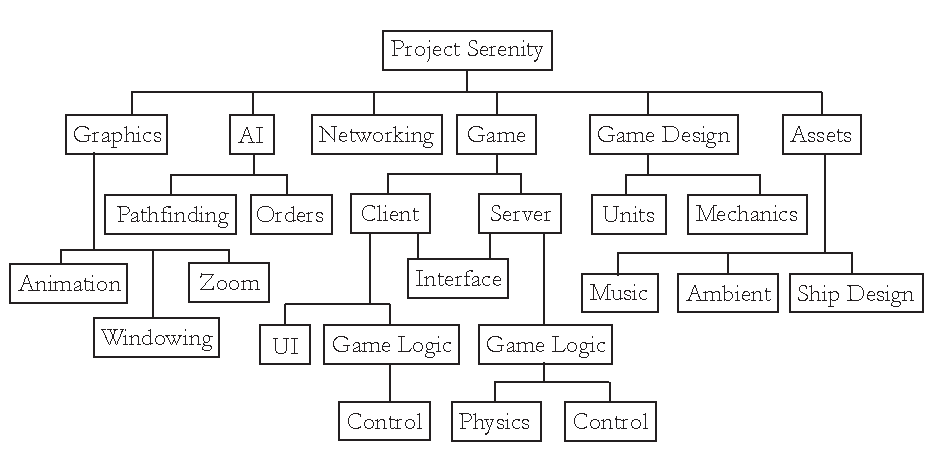
\includegraphics{res/wbs}
	\caption{Work Breakdown Structure of the game components.}
\end{figure*}

From the WBS we can further break the project down into components which are suited for weekly development cycles.

Term 2 releases will include a UI, an AI system and further improvements to the components as required. Assets such as music and additional ship designs are non-essential and will likely follow in a later release.

\begin{figure*}
	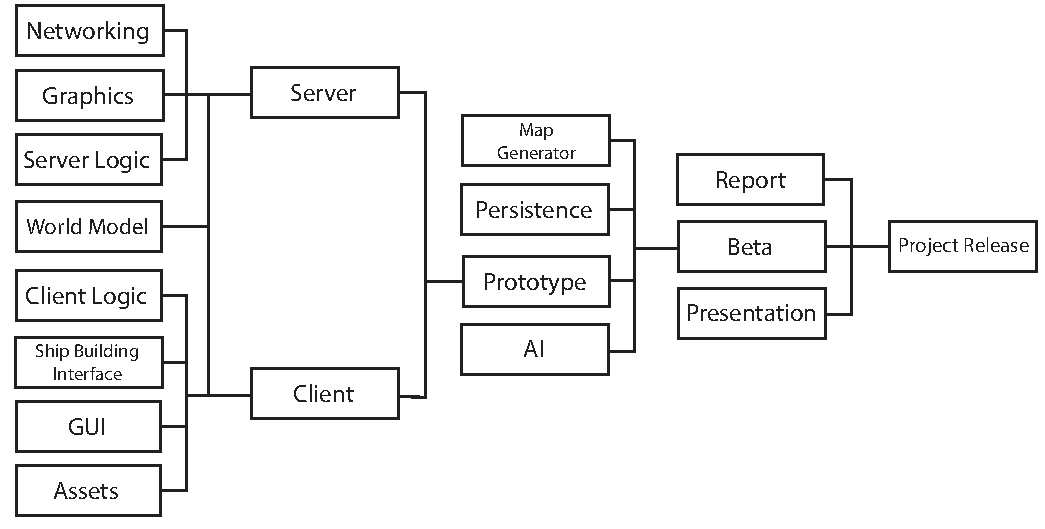
\includegraphics{res/dependency_tree}
	\caption[][-4.3em]{Component Dependency Graph.}
\end{figure*}

\begin{figure*}[h!]
	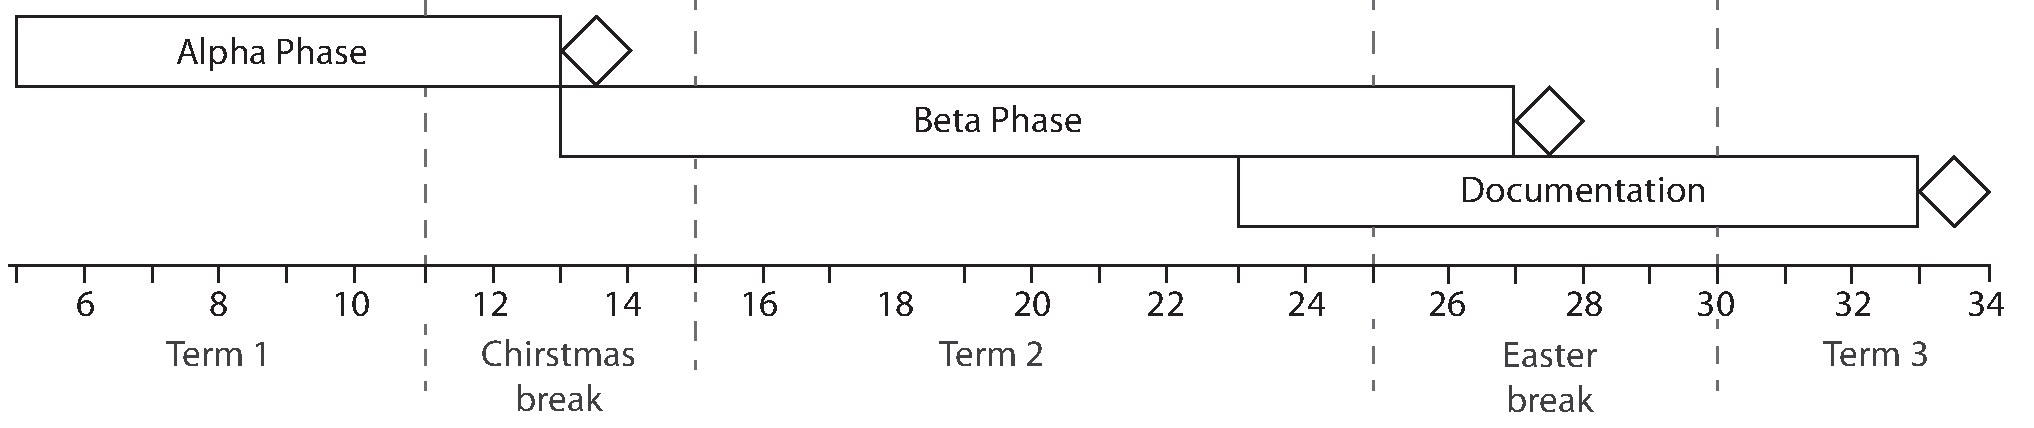
\includegraphics{res/gantt_chart_annotated}
	\caption{Phase level Gantt chart.}
\end{figure*}

The dependency tree shows which components are directly dependant on others, and show how delays will propagate through the project. The project dependency diagram shows that potential loss is minimised after a prototype is complete, that is to say there are fewer critical dependancies from the prototype level onwards. This information emphasises the priority of the server and client components should the project schedule require revising at a later stage.





\begin{figure}
	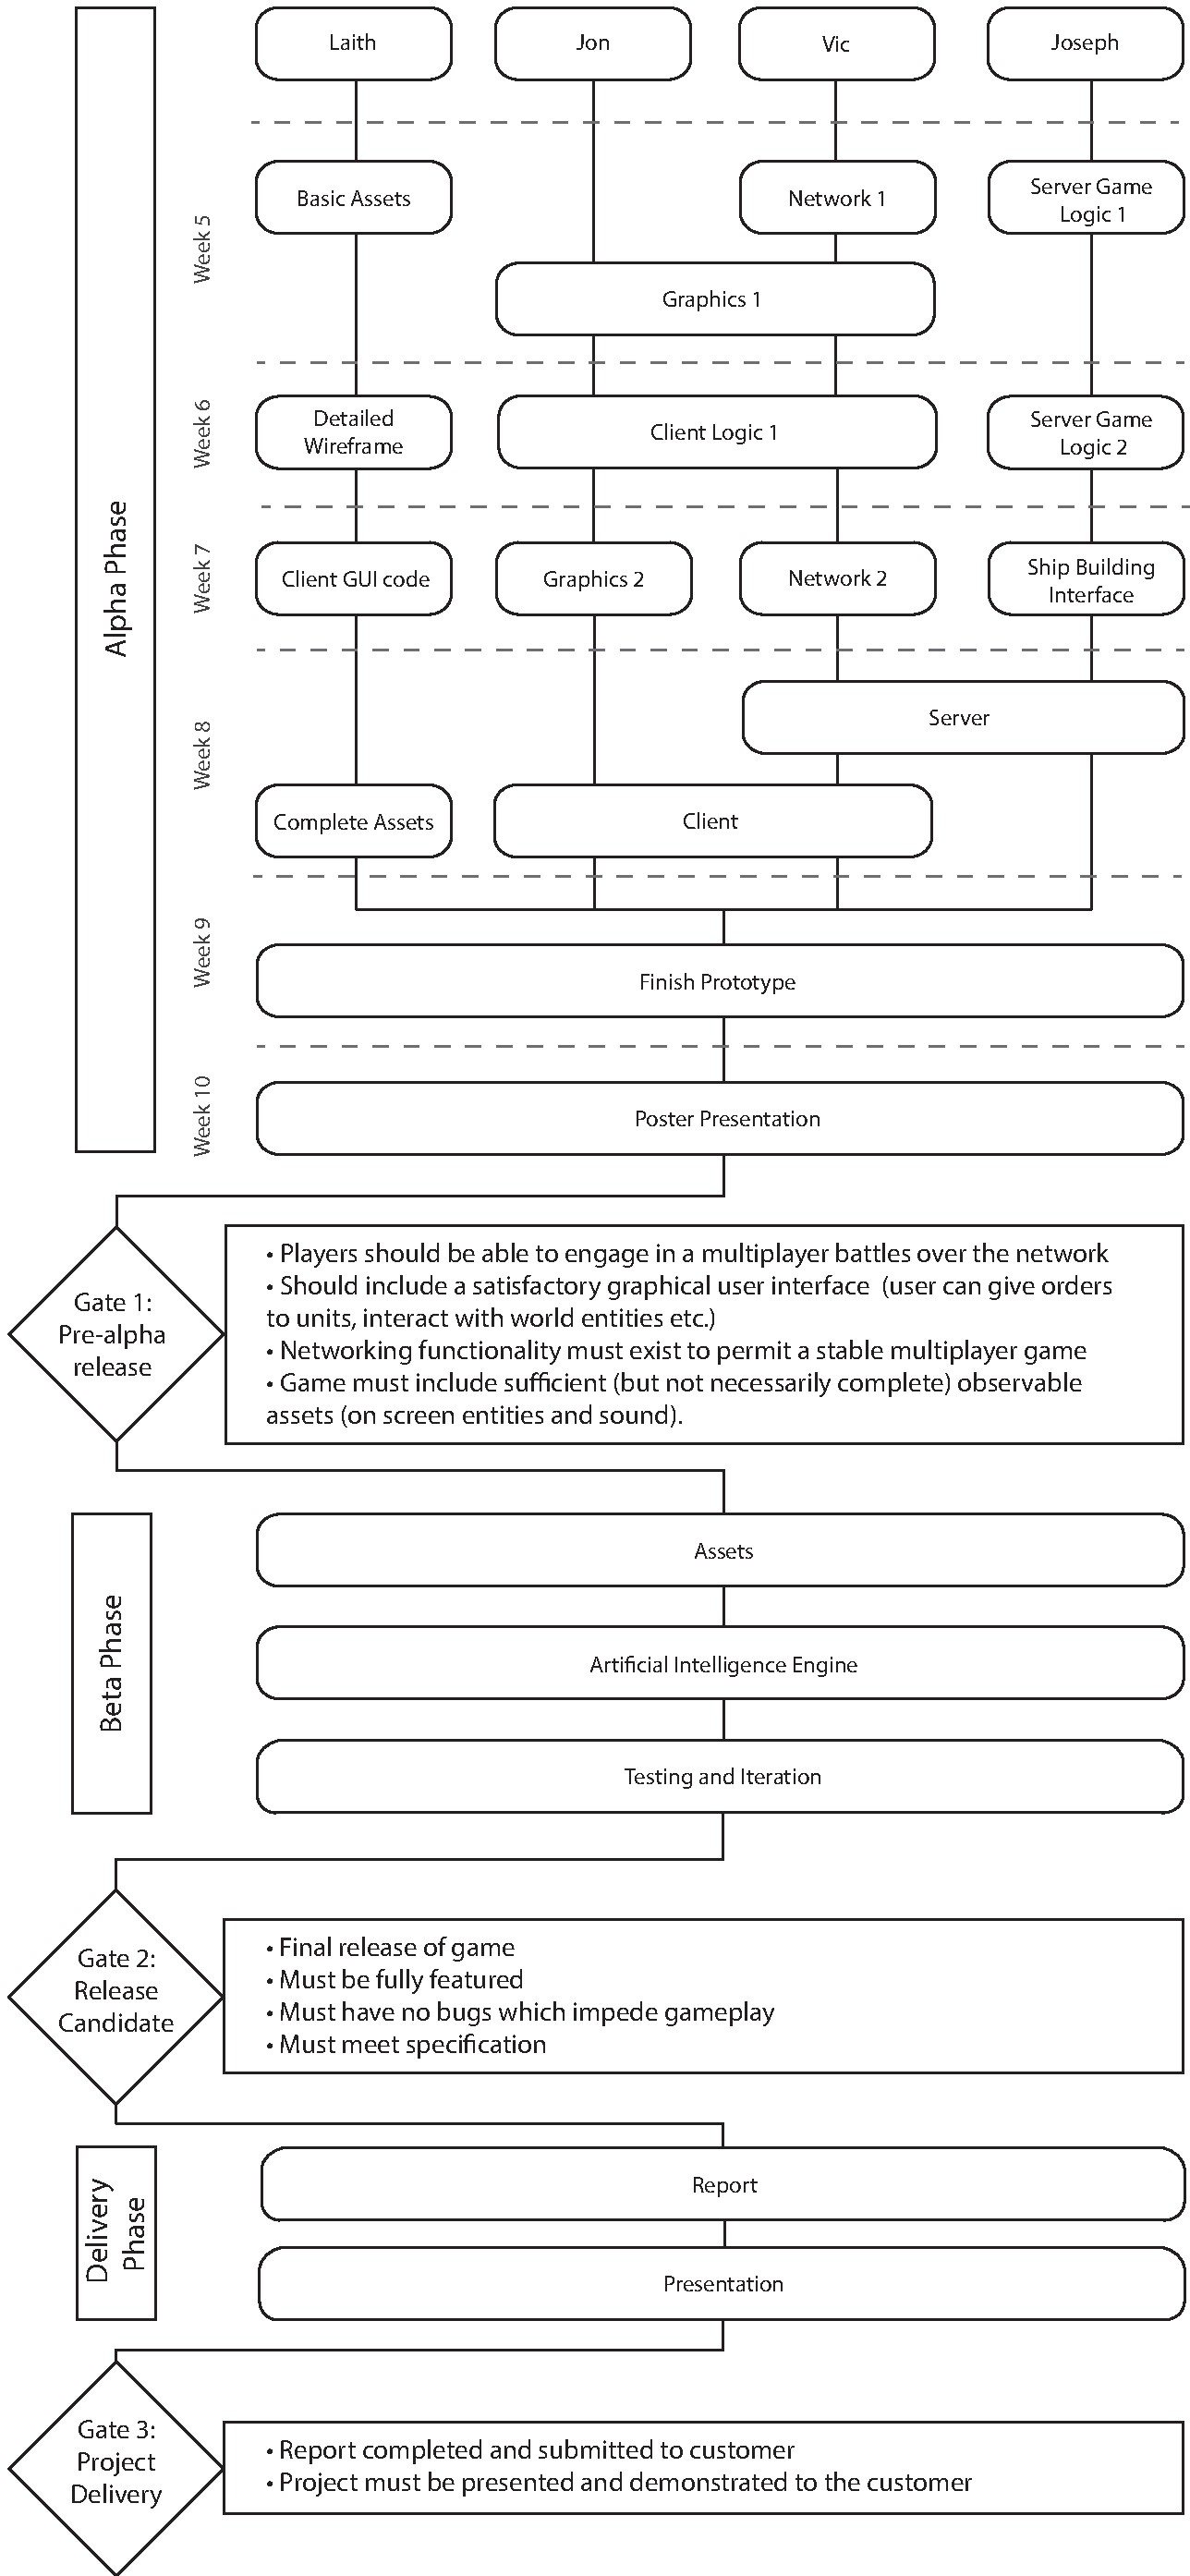
\includegraphics{res/stage_gate_diagram}
	\caption{Stage-gate model of work breakdown structure showing the division of labour across the various project phases. 
	The alpha phase is more thoroughly planned so we are able to see a weekly breakdown of tasks in the near future. The gates are project milestones, each of which details the requirements for proceeding through that gate into the next phase.}
\end{figure}

\section{Legal, Ethical, and Social Issues}
\label{section:professional_issues}

% legal
One potential legal issue faced by this project is the use of third party software.
It must be ensured that any third party libraries included in the code are licensed
appropriately. This means only using software with a permissive license (e.g. Apache, BSD, or MIT licenses) and no proprietary software.

Game publishers such as Electronic Arts, and Lion Head, consider their games as intelliectual property and copyright their games.
It is infeasible to check that all previous games published do not bear great similarities which could result in a court case.

% ethical
Games can be highly addictive, resulting in their players investing many hours into the game.
If the game is pay-to-play, this can also result in large sums of money invested into the game.
The game being developed uses a fixed length campaign of 5 battles, resulting in convenient game play periods for the user to quit the game.  

% social issues
The game is based in a fictional world, with a non-realistic graphical representation of this world. Current issues with games, such as racism, and violence are not an issue with this game.

The game will only support the english language.
This prevents users from using the game who cannot read english.




	\chapter[Project Management]{Project Management}
\label{ch:management}

\chapterepigraph{``All things are created twice; first mentally; then physically.  The key to creativity is to begin with the end in mind, with a vision and a blue print of the desired result."}{ Stephen Covey}

\newthought{Starting a sentence} with a new thought.

Our project team has adopted the agile development cycle as a basis for our management structure. We've broken the project down into critical components and have committed to weekly releases to ensure the project remains well scheduled throughout the project lifetime.

\section{Risk Management}
\label{section:risk}
 
A proactive approach to risk management was taken. This technique was chosen in order
to maximise the probability of avoiding risks instead of having to move into `fire-fighting mode'
if something went wrong.\citepage{pressman2010}{page 745}
 
As part of this proactive risk management strategy, a number of potential risks were identified.
These risks are shown in table~\ref{tab:risks} along with their estimated probabilities of occurring
and impact if they were to occur.
 
\begin{table*}
	\small
	\begin{tabular}{l p{\textwidth / 2} l l}
		\toprule
		\emph{Risk} & \emph{Description} & \emph{Probability} & \emph{Impact} \\
		\midrule
		Length underestimate & The time required to develop the software is underestimated & Medium & High \\
		Team member illness & One or more team members unable to work due to illness & Medium & High \\
		Hardware failure & Damage to critical hardware causing loss of data & Medium & Medium \\
		Size underestimate & The size of the deliverable has been underestimated & Medium & Medium \\
		Requirements change & Large number of changes to requirements during development & Low & Medium \\
		Ambiguous requirements & Requirements are not fully understood or misinterpreted leading to
			loss of development time as the specification is recreated & Low & Medium \\
		\bottomrule
	\end{tabular}
	\vspace{1.5em}
	\caption{Risk identification and analysis.}
	\label{tab:risks}
\end{table*}
 
With the risks identified, and their likelihood and consequences estimated it is necessary
to draw up plans to mitigate their effects. There are three types of management strategies 
for individual risks: avoidance strategies to reduce the probability of the risk occurring;
minimisation strategies to reduce the impact of the risk; and contingency plans to deal with
the risk if it does arise.\citepage{sommerville2011}{page 601} It is best to avoid the risk,
but if this is not possible then minimisation of the effects and, finally, contingency plans
should reduce the overall impact of a risk on the project. The mitigation and management
strategies for each risk previously identified are listed in table~\ref{tab:rmm}.
 
\begin{table*}
	\small
	\begin{tabular}{l p{37em}}
		\toprule
		\emph{Risk} & \emph{Mitigation / Management} \\
		\midrule
		Length underestimate & Detailed work breakdown with weekly releases to ensure that
			schedule slippage can be caught early \\
		Team member illness & Well documented code (enforced by the software librarian) so
			that other members can quickly start work on less familiar sections of
			the codebase \\
		Hardware failure & Backups and distributed source control, see section~\ref{section:tools} \\
		Size underestimate & Detailed work breakdown structure \\
		Requirements change & Thorough change management system, see section~\ref{section:control} \\
		Ambiguous requirements & Thorough planning phase \\
		\bottomrule
	\end{tabular}
	\vspace{1.5em}
	\caption{Risk mitigation and management.}
	\label{tab:rmm}
\end{table*}
 
The final stage of the risk management process is monitoring. Throughout the duration of
the project each identified risk was reassessed for changes to its probability and
impact. This allowed the mitigation and management strategies to be revisited to ensure that
they were as effective as possible.
 
The two previously identified risks that actually occurred were team member illness and length underestimate.
On a couple of occasions a team member was ill and unable to attend group work sessions or work to their full
capacity. Fortunately, the team was able to reduce the impact of this by ensuring that the work each individual
was performing was not hindered by an absence. This was done by allocating work tasks to be as separate as
possible to allow more parallel development to occur. Also, an illness was never so severe as to stop a team
member from working for longer than a day or two. However, the issue of length underestimation was more serious.
 
% Length underestimation
%
% 1. More time required for network and GUI than hoped
% 2. (1) slowed the development of the ideal game
% 3. (1) was very informative for our goal of investigation of Haskell for game development
 
The proactive approach to risk management was a good choice. By reviewing the potential
risks before starting the development phase of the project it was much easier to avoid risks that could
have had disastrous consequences for the project. For example, by implementing a thorough backup strategy
prior to any data loss actually taking place it was ensured that no work would have been lost if a hardware
failure had occurred. Continuously monitoring and reassessing these risks was also helpful in preventing
any risks becoming more probable or having a greater impact.

\section{Grievance Policy}
It's imperative to document a grievance guideline to ensure that any grievance procedures are fair and impartial. %ref gov
 Because the developer team is small, an internal dispute would have a high cost to the project, so grievance issues need to be dealt with promptly. 
  
\begin{enumerate}[i)]
    \item{Attempt to resolve the grievance issue informally by the team manager.}
    \item{If the issue cannot be resolved informally, and affects the entire project group, then address the issue at the next meeting and attempt to find a resolution in a group environment.}
    \item{If the issue cannot be solved by a formal group meeting then a managerial confrontation is required to reduce the impact on the project.}
    \item{If the issue still cannot be resolved then a complaint should be made to the module supervisor and university procedure should be followed from then on.}
\end{enumerate}

\section{Weekly Releases}
As a motivating factor to keep the project on schedule we've committed to component releases every Tuesday evening. The release should include the latest completed iteration of the project, which is scheduled to develop as a prototype by the end of term 1.

\section{Standup Meetings}
Standup meetings are held every week to discuss individual progress on the project, any issues an individual has been encountered, and what they will attempt to accomplish in the following week.

\section{Change Management}

\section{Tools and Techniques}

\section{Develop}

Whatever that means...
%\part{Research\label{part:research}}
%	\chapter[Current Trends in the Gaming Industry]{Current Trends in the Gaming Industry}
\label{ch:industry}

\chapterepigraph{``Perhaps it hasn't one," Alice ventured to remark. ``Tut, tut, child!" said the Duchess. ``Everything's got a moral, if only you can find it."}{from Lewis Carol's  \emph{Alice in Wonderland}}

\newthought{Starting a sentence} with a new thought.

\section{A Section}

Lorum ipsum dolor sit amet.

%	\chapter[Existing Games using Functional Programming Platforms]{Existing Games using Functional Programming Platforms}
\label{ch:existing_games}

\chapterepigraph{``Perhaps it hasn't one," Alice ventured to remark. ``Tut, tut, child!" said the Duchess. ``Everything's got a moral, if only you can find it."}{from Lewis Carol's  \emph{Alice in Wonderland}}

\newthought{Starting a sentence} with a new thought.

\section{A Section}

Lorum ipsum dolor sit amet.
%	\chapter[IO, Networking, and Graphics --- Tackling the Awkward Squad]{IO, Networking, and Graphics --- Tackling the Awkward Squad}
\label{ch:awkward}

\chapterepigraph{``Perhaps it hasn't one," Alice ventured to remark. ``Tut, tut, child!" said the Duchess. ``Everything's got a moral, if only you can find it."}{from Lewis Carol's  \emph{Alice in Wonderland}}

\newthought{Starting a sentence} with a new thought.

\section{A Section}

Lorum ipsum dolor sit amet.

%\part{Building the Game\label{part:main}}
%	\section{Networking}

% How the problems of game networking were solved in the network layer

Lorum ipsum sit dolor amet.\citefix{church1932}  \lipsum[2-4]	
%	\section{Graphics Programming in Haskell}

% OpenGL, Gloss etc

\begin{marginfigure}
	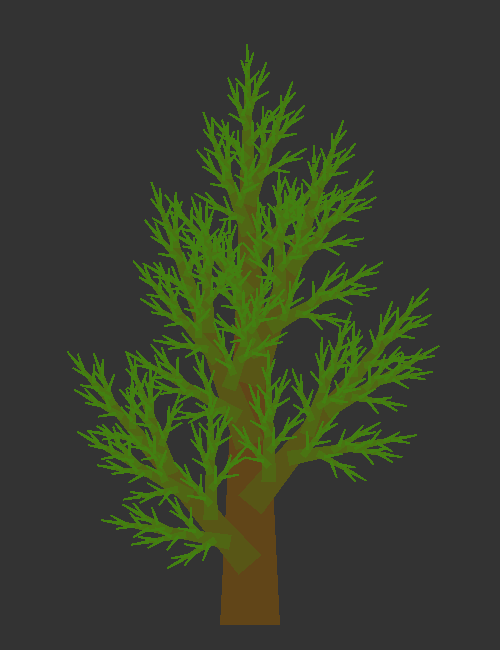
\includegraphics{res/gloss/gloss-tree.png}
	\vspace{1em}
	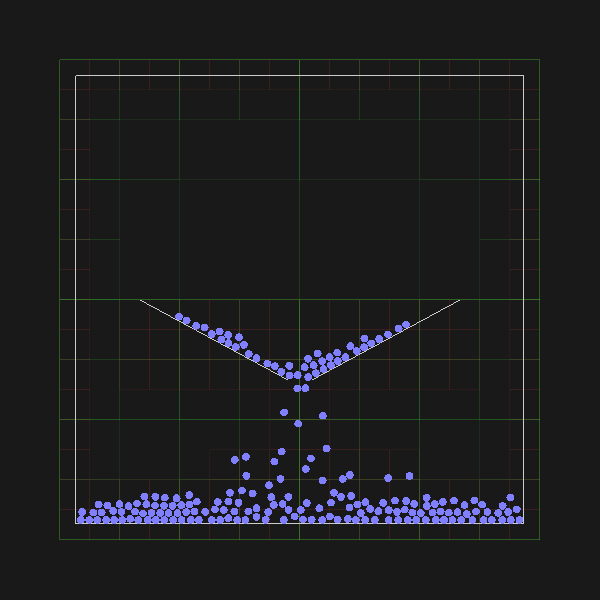
\includegraphics{res/gloss/gloss-styrene.png}
	\caption[Gloss example screens.]{Gloss example screens from \url{gloss.ouroborus.net/}.}
	\label{fig:gloss}
\end{marginfigure}

Any game is clearly going to involve graphics in some capacity or another, but graphics are not something that at first sight seem suited to a functional language. There are, however, various graphical frameworks and bindings available for Haskell.

For the purposes of the Serenity project, the choice basically boiled down to three options. Firstly, there are bindings directly to OpenGL available; which would provide the most flexibility but also likely the most development time. Secondly there are the bindings to the SDL engine, along with all the various tools provided with its framework. Many of the existing games written in Haskell use SDL. Lastly there is the use of the simple but effective layer over GLUT and OpenGL provided by the Gloss library.

This was not an easy decision, and some time went into making it. The direction taken in the Serenity project was to use the Gloss library, mostly because of its simple interface and ease of use, given the limited time and large scope of the rest of the project. The advantages of Gloss can be appreciated by considering the two screens in Figure \ref{fig:gloss}. Both of these examples involve relatively simple code, which is almost entirely pure.

The decision to use Gloss has largely been held up, but there has been some problems due to features it lacks, the most notable being clipping. In the future it would probably be beneficial to replace Gloss with an in house framework providing a layer between the pure graphics code and impure bindings to OpenGL.

Some details of the OpenGL and Gloss approaches are given below to illustrate the differences and tradeoffs involved.

\subsection{Using OpenGL Directly}

\marginnote{{\bf NB} --- The OpenGL code in this section is based on the tutorial at \url{haskell.org/haskellwiki/OpenGLTutorial1} (retrieved April 2013).}
Writing OpenGL code in Haskell is in many ways similar to writing it in C++ or any similar language. OpenGL calls are simply functions in the IO monad, (i.e. functions of type "IO a"), and there are some special primitive types such as "GLFloat". 

Listing~\ref{list:openglbasic} shows a very simple example of drawing an empty circle and a filled circle, and the output is shown in Figure~\ref{fig:openglbasicout}. Normal Haskell style is used to create a circle: using the "map" function and some trigonometry. These are then converted into OpenGL actions and rendered in the display callback. 

\vspace{-0.5em}
\begin{listing}{list:openglbasic}{Simple OpenGL example, drawing an empty circle and a filled circle (output shown in Figure~\ref{fig:openglbasicout}).}{Simple OpenGL example, drawing an empty circle and a filled circle (output shown in Figure~\ref{fig:openglbasicout}).}{}
\end{listing}\vspace{-1.5em}

\functions(myPoints, pointToVertex, renderMyPoints, display, main, flush, displayPrimitive, displayCallback, getArgsAndInitialize, mapM_, createWindow, mainLoop, clear, renderPrimitive)
\begin{haskell}

>import Graphics.Rendering.OpenGL
>import Graphics.UI.GLUT

>myPoints :: GLfloat -> [(GLfloat,GLfloat,GLfloat)]
>myPoints r = map (\k -> (r*sin(2*pi*k/n),r*cos(2*pi*k/n),0.0)) [1..n] 
>  where n = 100

>pointToVertex :: VertexComponent a => (a, a, a) -> IO ()
>pointToVertex (x,y,z) = vertex $ Vertex3 x y z

>renderMyPoints :: GLfloat -> IO ()
>renderMyPoints r = mapM_ pointToVertex (myPoints r)

>main = do 
>  (progname, _) <- getArgsAndInitialize
>  createWindow "OpenGL Example"
>  displayCallback $= display
>  mainLoop

>display = do 
>  clear [ColorBuffer]
>  renderPrimitive LineLoop (renderMyPoints 1)
>  renderPrimitive TriangleFan (renderMyPoints 0.5)
>  flush

\end{haskell}
\begin{marginfigure}[-25em]
	\hspace{-2em}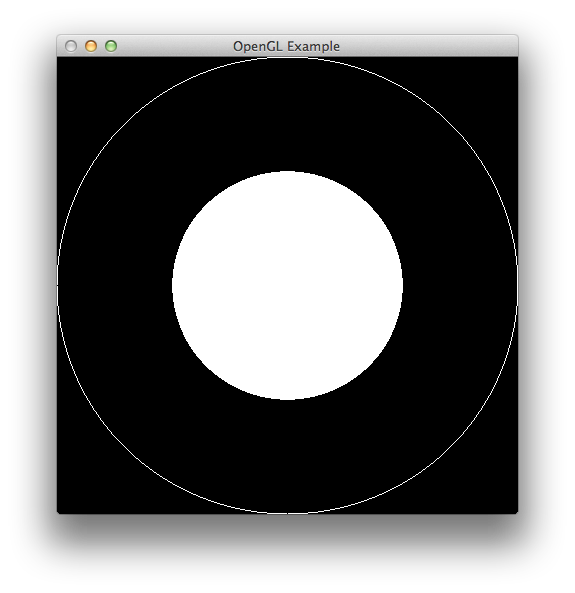
\includegraphics[width=18em]{res/opengl/openglbasic.png}
	\caption[Output of example OpenGL code in Listing~\ref{list:openglbasic}.]{Output of example OpenGL code in Listing~\ref{list:openglbasic}.}
	\label{fig:openglbasicout}
\end{marginfigure}
\vspace{-1em}
\noindent 
The challenge of programming graphics this way is far less an issue of language paradigm than it is of coding style: maintaining a proper separation between the concerns of basic rendering, specific entity models, the game logic, and so on, is the where main engineering effort is required --- and this is no different in Haskell than in other languages. 

As discussed in the previous section, there are various ways that such separation can be achieved, and that primary among these is the concept of an interim type. It is exactly this approach that is taken by the Gloss library, and this is the main reason Gloss was used in Project Serenity, to avoid the additional time it would take to build the infrastructure to work effectively with OpenGL.

\subsection{Using Gloss}

\begin{marginfigure}
	\hspace{-3em}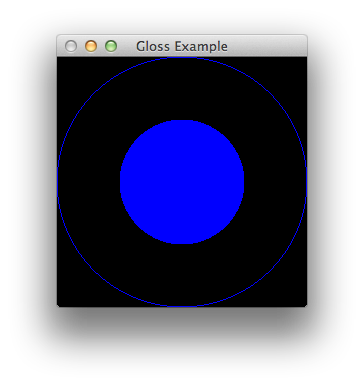
\includegraphics[width=21em]{res/gloss/glossbasic.png}
	\caption[Output of example Gloss code in Listing~\ref{list:glossbasic}]{Output of example Gloss code in Listing~\ref{list:glossbasic}.}
	\label{fig:glossbasicout}
\end{marginfigure}

Gloss is a layer that sits on top of OpenGL and GLUT providing a much simpler and cleaner API for drawing vector graphics. The Gloss project website claims that ``Gloss hides the pain of drawing simple vector graphics behind a nice data type and a few display functions'', and that using Gloss allows you to ``get something cool on the screen in under 10 minutes''.\sidenote[][1em]{See \url{hackage.haskell.org/package/gloss}} The simplicity of using Gloss compared to raw OpenGL code is shown in Listing~\ref{list:glossbasic} which recreates the simple OpenGL example in Gloss (although the colour of the circles has been changed to make the difference in outputs obvious).

\vspace{-0.5em}
\begin{listing}{list:glossbasic}{Example of simple Gloss usage}{Simple Gloss example, drawing an empty circle and a filled circle (output shown in Figure~\ref{fig:glossbasicout}).}{}
\end{listing}\vspace{-1.5em}

\functions(display, black, circles, color, blue, circleSolid, circle, play, playIO)
\begin{haskell}
>import Graphics.Gloss
>
>main = display (InWindow "Gloss Example" (250, 250) (0, 0)) black circles
>
>circles = Pictures $ map (color blue) [circleSolid 125, circle 250]

\end{haskell}
\noindent
This example simply creates a window named ``Gloss Example'' with a black background and adds the specified "Picture" to it. A "Picture" is the Gloss abstraction of the OpenGL primitives. In the example the picture to display is defined by the "circles" function.

The example in Listing~\ref{list:glossbasic} uses the "display" mode to draw a static picture to the screen. The game mode, started with "play" or "playIO", is obviously more useful when developing a game. It keeps track of a game world, the current state of the game, for which the developer provides callbacks for updating the world every tick and for converting the world to a "Picture". It also allows the programmer to add callbacks for handling input events such as mouse movement and clicks. The Gloss documentation and \texttt{gloss-examples} package are great sources of further information on getting started with game development with Gloss.\sidenote[][-5em]{See \url{hackage.haskell.org/package/gloss} and \url{hackage.haskell.org/package/gloss-examples}}

\subsection{Summary of this section} 
Given the limited time available for the Serenity project, the prebuilt pure interface onto OpenGL provided by the Gloss library was the best option, and this has been born out by the results. A custom made layer that is more appropriate for the needs of a complex game, and more readily adapted to changing requirements, would be beneficial to develop in the future.

%	\input{chapter/main/ai}
%	\section[Effective Unit Testing with Quickcheck and HUnit]{Effective Unit Testing with Quickcheck and \\HUnit}
\label{sec:testing}

% Find problems early
% Facilitates change

% \subsection{HUnit}

The HUnit library is the Haskell implementation of the standard xUnit unit testing framework. The
basic idea of the HUnit library is to provide the functions under test with some example data
and to compare the actual result with the expected result.

\vspace{-0.5em}
\begin{listing}{list:hunit}{Example usage of HUnit}{Example usage of HUnit. Testing a function that returns the length of a list.}{}
\end{listing}\vspace{-1.5em}

\functions(testEmpty, testTwo, tests, assertEqual, len)
\functions(runTestTT)
\begin{haskell}
>import Test.HUnit
>
>testEmpty = TestCase $ assertEqual "Empty list is zero" (len []) 0
>testTwo = TestCase $ assertEqual "List length two" (len [0, 1]) 2
>tests = TestList [testEmpty, testTwo]

\end{haskell}
\noindent An example of a small set of tests is shown in Listing~\ref{list:hunit}. This example shows
two simple tests for a function, "len", that returns the length of a given list.
A test, or list of tests, can be run with the use of the "runTestTT" function:

\begin{verbatim}
ghci> runTestTT tests
Cases: 2  Tried: 2  Errors: 0  Failures: 0
\end{verbatim}

% \subsection{QuickCheck}

\noindent Property based testing is a higher level approach to testing in which the programmer develops a specification
for the code to be testing. QuickCheck is a type-based property testing library that generates test
cases automatically from the developer defined expected properties.\cite{claessen2000} These properties
need to be true for all inputs to the function (i.e.\ invariants). This is an extremely
powerful approach to testing that allows the developer to write short testable specifications that
are used to verify the code with thousands of test cases which would be infeasible to write by hand.

\vspace{-0.5em}
\begin{listing}{list:quickcheck}{Example usage of QuickCheck}{Example usage of QuickCheck. Properties of a function that returns the absolute value of a number.}{}
\end{listing}\vspace{-1.5em}

\functions(prop_NonNegativity, prop_Multiplicativeness, prop_Subadditivity, prop_Idempotence, prop_Symmetry, absolute)
\functions(quickCheck, quickCheckWith, maxSuccess, verboseCheck)
\begin{haskell}
>import Test.QuickCheck
>
>prop_NonNegativity x = absolute x >= 0
>prop_Multiplicativeness x y = absolute (x * y) == (absolute x) * (absolute y)
>prop_Subadditivity x y = absolute (x + y) <= (absolute x) + (absolute y)
>prop_Idempotence x = absolute (absolute x) == absolute x
>prop_Symmetry x = absolute (-x) == absolute x

\end{haskell}
\noindent Listing~\ref{list:quickcheck} shows an example use case of QuickCheck to define five properties
of a function, "absolute", that returns the absolute value of a given number. The tests can then
be run by invoking the "quickCheck" function on one of the properties, for example:

\begin{verbatim}
ghci> quickCheck (prop_NonNegativity :: Integer -> Bool)
+++ OK, passed 100 tests.
\end{verbatim}

\noindent
This means that for one hundred randomly generated test cases the property held. It is
possible to get QuickCheck to run a different number of tests by using the "quickCheckWith"
function and specifying a different number for the "maxSuccess" argument. The actual
test cases that were generated can be viewed by using "verboseCheck" instead of "quickCheck"
--- be warned that, as the name implies, this is very noisy!

Testing is another area where the separation of pure and impure code becomes very useful.
By using the techniques laid out in the previous sections it is possible to have the majority
of game logic in pure functional code. This is of great benefit when it comes to testing
because, as Claessen and Hughes state, ``functional programs are well suited to automatic
testing''.\cite{claessen2000} Referentially transparent functions are much easier to test
than those that produce side-effects because program state before and after execution
is a nonissue.

During the development of the Serenity project an effective testing method combining the
use of QuickCheck and HUnit was found. QuickCheck was used to generate large numbers of
test cases for individual pure functions, and HUnit for impure functions, such as network
code, and units of code comprised of several functions used together. This approach allows
using the powerful property based testing where applicable in conjunction with more specific
HUnit test cases to maximise test coverage and confidence that the expected results are
being produced.

% Example from Serenity

\subsection{Organising an automated test suite}

When creating a test suite for your software project it is useful to organise it in such
a way as to allow quick automated testing, i.e.\ being able to run the entire test suite
with a single command. The easiest way to do this in a Haskell project is to use the
\texttt{test-framework} library. This library enables the user to group lists of tests
into cohesive units and then run a list of tests and test groups with a single function
call.

\vspace{-0.5em}
\begin{listing}{list:testframework}{Running tests with test-framework}{Running tests with test-framework}{}
\end{listing}\vspace{-1.5em}

\functions(main, defaultMain, allTests)
\begin{haskell}
>import Test.Framework
>
>main = defaultMain allTests
>
>allTests =
> [ Packet.tests
> , Transport.tests
> , Message.tests
> -- ...
> , MathUtil.tests
> ]

\end{haskell}
\noindent Listing~\ref{list:testframework} is an extract from the main entry point to
the Serenity test suite. It creates a list of tests from the test groups exported by
individual test modules. These tests are run by the "defaultMain" function provided by
"Test.Framework".

Grouping HUnit and QuickCheck tests with \texttt{test-framework} requires the use of
two further libraries, \texttt{test-framework-hunit} and \texttt{test-framework-quickcheck2}.
These two libraries provide functions to convert HUnit assertions and QuickCheck properties
into the "Test" type used by \texttt{test-framework}. A brief example of their use
in Serenity to build a group of tests to export is shown in Listing~\ref{list:testgroup}.

\vspace{-0.5em}
\begin{listing}{list:testgroup}{Grouping tests with test-framework}{Grouping tests with test-framework}{}
\end{listing}\vspace{-1.5em}

\functions(testGroup, testCase, testProperty, testReadNTChan, testReadTChanUntilEmpty, prop_EmptyTChan)
\begin{haskell}
>import Test.Framework (testGroup)
>import Test.Framework.HUnit (testCase)
>import Test.Framework.QuickCheck2 (testProperty)
>
>tests = testGroup "Network utility tests"
> [ testCase "Test readNTChan" testReadNTChan
> , testCase "Test readTChanUntilEmpty" testReadTChanUntilEmpty
> , testProperty "Empty TChan" prop_EmptyTChan
> ]

\end{haskell}
\noindent
A test suite organised with the \texttt{test-framework} module can be easily integrated into the
Cabal build system.\sidenote{See \url{http://www.haskell.org/cabal/users-guide/developing-packages.html\#test-suites}}
For example, here is the additional configuration added to the \texttt{Serenity.cabal}
file to enable a Cabal backed test suite:

\begin{verbatim}
Test-Suite test-serenity
  type: exitcode-stdio-1.0
  hs-source-dirs: tests, src
  main-is: Main.hs
  build-depends:
    -- ... list of dependencies
\end{verbatim}

\noindent
The cabal-install program will look in \texttt{Main.hs} to find the "main" function
which runs the entire suite of tests.
With this test suite definition in place only a few commands a required to
configure the project with the tests enabled, build it, and run the entire suite:

\begin{verbatim}
# cabal configure --enable-tests
# cabal build
# cabal test
\end{verbatim}

This set up allows easy use of a build server to run the test suite whenever a change
is pushed to a master version control repository. For the Serenity project an instance
of the Jenkins continuous integration server was set up for this purpose.\sidenote{See Section~\ref{sec:tools}}
Jenkins allows the user to specify a shell script to execute when building the project.
During the development of Serenity the following script was used to automatically run
the test suite:

\begin{verbatim}
set -e
cd '$WORKSPACE/Serenity/'
cabal update
cabal install --only-dependencies --avoid-reinstalls --enable-tests
cabal clean
cabal configure --enable-tests
cabal build
cabal test
\end{verbatim}

\noindent
Using this script the build server installs any new dependencies and then runs the
entire test suite. Using a build server to run the test suite on every change is a
good method of running the tests regularly to help find any errors early in the
development cycle.

\subsection{Test driven development}

Test driven development (TDD) is a practice in software development that promotes testing
by writing tests before implementing the functionality that it tests. The TDD cycle
proposed by Kent Beck has five steps:\cite{beck2003}

\begin{enumerate}
\item Add a test that defines the new functionality. By writing the test before starting on
	the implementation the developer is forced to clearly understand the requirements of
	the new feature and think about some design aspects before rushing into coding,
	such as the API of a new function.

\functions(newFunction)
\item Run all tests to watch the new test fail. Since the implementation has not been written
	yet the new test must fail, but running the test suite now has two benefits. Firstly
	it checks that the new test is not worthless by always passing. Secondly it ensures
	that the test suite is run frequently causing the code to be exercised often.\sidenote{Note that the code might not even compile now since the new function under test is not defined. To remedy this the developer can do the least that is required to get the system compiling again, e.g.\scalenote{"newFunction = undefined"}}

\item Write the minimal amount of code required to make the new test pass. This code is not
	supposed to be perfect, but the simplest implementation to pass the test.

\item Run the tests to watch the new test succeed; the naive implementation passes the tests.
	This is a good baseline to start improving the code from.

\item Refactor the new code. The implementation can now be improved to make sure that it is
	of production quality. The test suite can be used to prove that the refactor is not
	changing the functionality of the code.
\end{enumerate}

This cycle can then be repeated with a new test for a new piece of functionality.
TDD also has good support for regression testing. If a bug is discovered then the developer
tasked with fixing it would write a test to reproduce the bug before fixing the current
implementation. In this way the set of test cases is broadened to cover even more
possible code paths and to ensure that previous bugs are not reintroduced by future
changes.

This is an approach to development advocated by the Serenity project team, and a core
development technique that was attempted during the project,\sidenote{See Section~\ref{sec:devmodel}}
for a number of reasons. Firstly, following TDD ensures that a project has a large
test suite with a good coverage of the code base because functions should not be
implemented without a test being written first. This is highly beneficial because
it shows that the software is reliable and it gives developers confidence that their
changes are not damaging the functionality of existing code. The 2005 study by
Erdogmus et al.\ supports this as they found that when adhering to the test-first
nature of TDD ``programmers write more tests per unit of programming effort'' and
that, in turn, more tests lead to an increase in productivity.\cite{erdogmus2005}
A second benefit for TDD is suggested by Sommerville who states that TDD ``helps
programmers clarify their ideas of what a code segment is actually supposed to
do''.\citepage{sommerville2011}{page 222} This is because constructing the test for
a new piece of functionality involves thinking about its requirements and design.

% Especially effective with CI

% \subsection{Behaviour driven development with hspec} Maybe?

%	\input{chapter/main/manual}
%\part{Project Evaluation\label{part:evaluation}}
%	\input{chapter/evaluation/game}	
%	\input{chapter/evaluation/haskell}
%	\chapter[Project Management]{Project Management}
\label{ch:management}

\chapterepigraph{``All things are created twice; first mentally; then physically.  The key to creativity is to begin with the end in mind, with a vision and a blue print of the desired result."}{ Stephen Covey}

\newthought{Starting a sentence} with a new thought.

Our project team has adopted the agile development cycle as a basis for our management structure. We've broken the project down into critical components and have committed to weekly releases to ensure the project remains well scheduled throughout the project lifetime.

\section{Risk Management}
\label{section:risk}
 
A proactive approach to risk management was taken. This technique was chosen in order
to maximise the probability of avoiding risks instead of having to move into `fire-fighting mode'
if something went wrong.\citepage{pressman2010}{page 745}
 
As part of this proactive risk management strategy, a number of potential risks were identified.
These risks are shown in table~\ref{tab:risks} along with their estimated probabilities of occurring
and impact if they were to occur.
 
\begin{table*}
	\small
	\begin{tabular}{l p{\textwidth / 2} l l}
		\toprule
		\emph{Risk} & \emph{Description} & \emph{Probability} & \emph{Impact} \\
		\midrule
		Length underestimate & The time required to develop the software is underestimated & Medium & High \\
		Team member illness & One or more team members unable to work due to illness & Medium & High \\
		Hardware failure & Damage to critical hardware causing loss of data & Medium & Medium \\
		Size underestimate & The size of the deliverable has been underestimated & Medium & Medium \\
		Requirements change & Large number of changes to requirements during development & Low & Medium \\
		Ambiguous requirements & Requirements are not fully understood or misinterpreted leading to
			loss of development time as the specification is recreated & Low & Medium \\
		\bottomrule
	\end{tabular}
	\vspace{1.5em}
	\caption{Risk identification and analysis.}
	\label{tab:risks}
\end{table*}
 
With the risks identified, and their likelihood and consequences estimated it is necessary
to draw up plans to mitigate their effects. There are three types of management strategies 
for individual risks: avoidance strategies to reduce the probability of the risk occurring;
minimisation strategies to reduce the impact of the risk; and contingency plans to deal with
the risk if it does arise.\citepage{sommerville2011}{page 601} It is best to avoid the risk,
but if this is not possible then minimisation of the effects and, finally, contingency plans
should reduce the overall impact of a risk on the project. The mitigation and management
strategies for each risk previously identified are listed in table~\ref{tab:rmm}.
 
\begin{table*}
	\small
	\begin{tabular}{l p{37em}}
		\toprule
		\emph{Risk} & \emph{Mitigation / Management} \\
		\midrule
		Length underestimate & Detailed work breakdown with weekly releases to ensure that
			schedule slippage can be caught early \\
		Team member illness & Well documented code (enforced by the software librarian) so
			that other members can quickly start work on less familiar sections of
			the codebase \\
		Hardware failure & Backups and distributed source control, see section~\ref{section:tools} \\
		Size underestimate & Detailed work breakdown structure \\
		Requirements change & Thorough change management system, see section~\ref{section:control} \\
		Ambiguous requirements & Thorough planning phase \\
		\bottomrule
	\end{tabular}
	\vspace{1.5em}
	\caption{Risk mitigation and management.}
	\label{tab:rmm}
\end{table*}
 
The final stage of the risk management process is monitoring. Throughout the duration of
the project each identified risk was reassessed for changes to its probability and
impact. This allowed the mitigation and management strategies to be revisited to ensure that
they were as effective as possible.
 
The two previously identified risks that actually occurred were team member illness and length underestimate.
On a couple of occasions a team member was ill and unable to attend group work sessions or work to their full
capacity. Fortunately, the team was able to reduce the impact of this by ensuring that the work each individual
was performing was not hindered by an absence. This was done by allocating work tasks to be as separate as
possible to allow more parallel development to occur. Also, an illness was never so severe as to stop a team
member from working for longer than a day or two. However, the issue of length underestimation was more serious.
 
% Length underestimation
%
% 1. More time required for network and GUI than hoped
% 2. (1) slowed the development of the ideal game
% 3. (1) was very informative for our goal of investigation of Haskell for game development
 
The proactive approach to risk management was a good choice. By reviewing the potential
risks before starting the development phase of the project it was much easier to avoid risks that could
have had disastrous consequences for the project. For example, by implementing a thorough backup strategy
prior to any data loss actually taking place it was ensured that no work would have been lost if a hardware
failure had occurred. Continuously monitoring and reassessing these risks was also helpful in preventing
any risks becoming more probable or having a greater impact.

\section{Grievance Policy}
It's imperative to document a grievance guideline to ensure that any grievance procedures are fair and impartial. %ref gov
 Because the developer team is small, an internal dispute would have a high cost to the project, so grievance issues need to be dealt with promptly. 
  
\begin{enumerate}[i)]
    \item{Attempt to resolve the grievance issue informally by the team manager.}
    \item{If the issue cannot be resolved informally, and affects the entire project group, then address the issue at the next meeting and attempt to find a resolution in a group environment.}
    \item{If the issue cannot be solved by a formal group meeting then a managerial confrontation is required to reduce the impact on the project.}
    \item{If the issue still cannot be resolved then a complaint should be made to the module supervisor and university procedure should be followed from then on.}
\end{enumerate}

\section{Weekly Releases}
As a motivating factor to keep the project on schedule we've committed to component releases every Tuesday evening. The release should include the latest completed iteration of the project, which is scheduled to develop as a prototype by the end of term 1.

\section{Standup Meetings}
Standup meetings are held every week to discuss individual progress on the project, any issues an individual has been encountered, and what they will attempt to accomplish in the following week.

\section{Change Management}

\section{Tools and Techniques}

\section{Develop}

Whatever that means...
%\part{Into the Future\label{part:future}}
%	\input{chapter/future/library}
%	\input{chapter/future/game}
%
%\part{Appendices and Indices\label{part:appendices}}
%
%\backmatter
%
%\chapter{Acknowledgements}

LOL

\begin{fullwidth}

\def\bibname{Full Reference List and Selected Bibliography}
\nocite{*}
\bibliographystyle{plainnat}
\addcontentsline{toc}{chapter}{\bibname}
\bibliography{references}

%\cleardoublepage
%\phantomsection \label{listoflis}
%\addcontentsline{toc}{chapter}{List of Listings}
%\listofvlisting
%
%\cleardoublepage
%\phantomsection \label{listoffig}
%\addcontentsline{toc}{chapter}{List of Figures}
%\listoffigures
%
\end{fullwidth}
%\printindex

\end{document}
